%% ================================================================================
%% This LaTeX file was created by AbiWord.                                         
%% AbiWord is a free, Open Source word processor.                                  
%% More information about AbiWord is available at http://www.abisource.com/        
%% ================================================================================
\documentclass[a4paper,12pt]{article}
\usepackage[latin1]{inputenc}
\usepackage{calc}
\usepackage{setspace}
\usepackage{graphicx}
\usepackage{multicol}
\usepackage{natbib}
\usepackage{amsmath}
%\usepackage[normalem]{ulem}
%% Please revise the following command, if your babel
%% package does not support en-US
%\usepackage{babel}
\usepackage{color}
\usepackage{hyperref}
 
 \author{Iva Babukova 2030458}
 
\title{Computational Study of the Travelling Salesman Problem}

\begin{document}

% \setlength{\oddsidemargin}{0.9847in-1in}
% \setlength{\textwidth}{\paperwidth - 0.9847in-0.9847in}

  
\maketitle


%%%%%%%%%% List of papers to review:
% 1. Dantzig, Fulkerson, Johnson 1954 --DONE
% 2. Sweeney at all: the B and B method --DONE
% 3. Held and Karp: The TSP and minimum spanning trees 1970 --DONE
% 4. Lin, Kernighan: An effective heuristic algorithm for the TSP 1973 --DONE
% 5. Small TSPs with CP --DONE
% 6. Relation between TSP and the longest path problem --DONE
%%%%%%%%%%

\section{Introduction and Problem statement}
The Travelling Salesman Problem (TSP) can be formulated as follows.
Given a set of $n$ cities $A$ with distance $d_{i,j}$ between each two cities $i$ and $j$ in $A$, A cycle of size $n$ through each city in $A$ is also called a \textit{tour}. TSP asks for finding a tour with minimum total sum of the distances between each pair of consecutive cities.

TSP has direct application in multiple fields: transportation and logistics \citep{Flood56}, planning inspections of remote sites \citep{Mahalanobis}, genome sequencing \citep{genomesequencing}, computer chips manufacturing \citep{Barbagallo96}, data clustering \citep{McCormick72} and many others. This implies a high demand in finding an efficient algorithm to solve TSP.

\citet{Flood56} conjectures that ``...there may well be no general method for treating the problem.'' This statement is later proved by \citet{thebible} who show that TSP is NP-hard. % In fact, there may well be no general method for treating the problem and impossibility results would also be valuable.''
The complexity of TSP and the high applicability of the problem in multiple fields has led to the development of more than 60 years old research in this area.

This work is a survey of six algorithms for TSP that represent the variety of existing algorithms for TSP. The fundamental work of \citet{Dantzig54} is first discussed in Section \ref{sec:dantzig54}. Section \ref{sec:bandb} is a review of branch and bound algorithms, where two particular techniques are discussed in Section \ref{subsec:little63} and Section \ref{sec:heldandkarp}. Section \ref{sec:tspwithcp} presents a Constraint Programming algorithm for TSP. Section \ref{sec:linkernighan} discusses a technique for repeatedly improving a sub-optimal tour within a given time limit. Section \ref{sec:tspandlpp} presents a method for reducing TSP to another NP-hard problem.

\section{Dantzig, Fulkerson and Johnson}
\label{sec:dantzig54}
\citet{Dantzig54} represent TSP as a system of linear integer inequalities, based on earlier work by \citet{heller53} and \citet{kuhn55}. The formulation is as follows.

Let $p$ be a tour in a TSP instance $\pi$ and let $x_{i,j}$ be 1 if $i$ is succeeded by $j$ in the tour or 0 otherwise, for $i,j \in A$ . Since TSP asks for a cycle of the cities in $A$, each city in $p$ has to be both preceded and succeeded by one city. \citet{Dantzig54} enforce this with the following constraint:

\begin{equation}
\label{eq:one}
\begin{split}
  \sum_{j \in A} x_{i,j} = 1, \qquad i \in A,\\
  \sum_{i \in A} x_{i,j} = 1, \qquad j \in A,
\end{split}
\end{equation}

Note that constraint (\ref{eq:one}) allows for cycles in $p$ of size $n_{1} < n$, also called \textit{subtours}, since each city can still have only one preceding and one succeeding city in such arrangements. To filter out subtours, \citet{Dantzig54} add the \textit{subtour elimination} constraint:

\begin{equation}
\label{eq:subtourElimination}
\sum_{S} x_{i,j} \leq n_{1} - 1, \qquad \forall S \subset A; \, n_{1} = |S| > 0; \, i,j \in S
\end{equation}

Equation (\ref{eq:subtourElimination}) restricts that the sum of $x_{i,j}$ over all $n_{1}$ cities in a subset $S$ of $A$ has to be less than $n_{1}$, which combined with constraint (\ref{eq:one}) restricts all cities in $S$ to be connected with at least one city not in $S$.

TSP is then formulated as the problem of minimising:

\begin{equation}
\label{eq:objfunc}
\sum_{i\in A}\sum_{j\in A} d_{i,j}x_{i,j}
\end{equation}

subject to constraints (\ref{eq:one}) and (\ref{eq:subtourElimination}).

The solution procedure is explained in the next paragraphs. It follows a branch and bound technique. Although the branch and bound method was coined by \citet{Little63}, it is believed that \citet{Dantzig54} is the first work that uses it \citep{tspbible}. Interestingly, the paper does not emphasise on this invention, but focuses more on one of the procedures in the algorithm, called the \textit{cutting planes} method, which is described later.

Let $\pi^{\prime}$ be the problem consisting of minimising function (\ref{eq:objfunc}) subject to constraint (\ref{eq:one}) only. From the properties of subtours, each solution to $\pi$ as a solution to $\pi^{\prime}$, however a solution to $\pi^{\prime}$ need not be a solution to $\pi$ \citep{Dantzig54}. \citet{Dantzig54} call $\pi^{\prime}$ a \textit{relaxation} of $\pi$ and use it as part of the branch and bound procedure to compute the lower bound on the tour length, using the algorithm of \citet{Kuhn55a} which has complexity $\mathcal{O(n^{3})}$.

This relaxation has great impact on the research in algorithms for NP-hard problems in general and it is still studied nowadays \citep{Cheung05}. Relaxations to other problems are defined and successfully used for various NP-hard problems \citep{Fisher04,Cruz10,Christofides81}. A possible reason why the field of problem relaxations flourished could be that this method has good performance in general and it allows for the reuse of already existing efficient algorithms to solve the relaxation.

TSP is then solved as follows:
\begin{enumerate}
\item Solve $\pi^{\prime}$, obtain a path $P^{\prime}$. Go to Step 2.
\item %While constraint (\ref{eq:subtourElimination}) is violated at some point of the tour: fix the tour by imposing the constraint for this point of the tour only.
If $P^{\prime}$ does not contain a subtour: go to Step 3. If $P^{\prime}$ contains a subtour $S$: impose constraint (\ref{eq:subtourElimination}) on $S$ and obtain a new path $P^{\prime\prime}$. $P^{\prime}$ = $P^{\prime\prime}$. Go to Step 2.
\item Output $P^{\prime}$, it is the optimal solution and terminate the program.
\end{enumerate}

Note that there were no computer resources available and \citet{Dantzig54} executed this algorithm by hand for the 49-city instance. The procedure steps are outlined in the paper through a series of small examples and the authors prove that it outputs an optimal tour.

Step 2 is the \textit{cutting planes} method. It consists of imposing the elimination constraint only to eliminate subtours of the initially computed path. \citet{Applegate07} observe that ``... the TSP literature from 1950s does not include any attempts to automate the \citet{Dantzig54} solution procedure...''. \citet{Dantzig59} write: ``... judging from the number of queries we have received from readers, this method was not elaborated sufficiently to make the proposal clear...'' and present a thorough explanation of the cutting planes method. This suggests that the reason for the low utilization of the cutting planes method in subsequent work is that it was not well understood by other researches in the field. 

The work of \citet{Dantzig54} was a computational record for more than 20 years. One of the algorithms capable of solving instances with more than 2000 cities, introduced by \citet{Padberg91} is based on the work of \citet{Dantzig54}.

The work of \citet{Dantzig54} is described as a ``breakthrough'' that ``...has reached far beyond the narrow confines of the TSP...'' \citep{Applegate07}. This method sets a standard for modelling not only TSP instances, but also instances of other problems \citep{Laporte86,Baker83,Agarwal89}.


\section{Branch and Bound Algorithms}
\label{sec:bandb}

\citet{Lawler66} refer to branch and bound methods as ``intelligently structured search of the space of all feasible solutions'. Starting with the set of all feasible solutions, the set is partitioned into successively smaller subsets, also called \textit{subproblems}, according to a specific \textit{branching rule}. A lower bound is calculated for the cost for each set of subproblems. Subproblems with bound that exceeds the lowest bound $l^{\star}$ found so far are discarded from the subproblem set. Otherwise, the subproblems are further partitioned. The procedure terminates when the subproblems can not be further partitioned and outputs the solution with bound equal to $l^{\star}$.

The performance of branch and bound algorithms depends on the choice of branching rule and bounding algorithm \citep{Christofides81,Lawler66}. The next two sections present two different techniques for this.

\subsection{The Branch and Bound method by Little, Murty, Sweeny and Caroline}
\label{subsec:little63}

Although \citet{Dantzig54} use branch and bound algorithm as an extension of the cutting plane method, this technique is coined by \citet{Little63}.

\subsubsection*{Branching}
The branching procedure can be represented as a rooted binary tree $T$, where the root of $T$ represents all possible tours and each intermediate node is a partial tour. Each node $X$ has two children: $Y$ and $\neg Y$, which split the tours into two disjoint sets, based on whether a pair of cities is contained in the tours or not. For instance, let $X$ be partitioned with respect to the pair of cities $(i,j)$. Then $Y$ represents all tours that visit city $j$ immediately after city $i$ and $\neg Y$ represents all other tours. The branching is done for every pair of cities and it will eventually yield complete tours.

Since there are $n$ cities, there are $n!$ possible tours, which is equal to the number of leaf nodes in $T$. From properties of binary trees, the number of nodes in $T$ in the worst case is $2n! - 1$. Therefore, if the lower bound on the tour distance is not tight enough and if the choice of the next pair of cities to be branched on is poor, the branching procedure will visit $2n! - 1$ states.

Let $D$ be an $n \times n$ matrix containing the distance between each pair of cities in $A$. To avoid the worst case scenario, \citet{Little63} split $X$, such that $Y$ is likely to include an optimum and $\neg Y$ unlikely to include it by choosing next pair of cities $(i,j)$ for $Y$ that have smallest distance in the reduced version of $D$. The reduction procedure is explained in the next section.

\subsubsection*{Lower Bounds}

The lower bound on the tours $\omega(\star)$ is obtained using the following reduction of the distance matrix $D$. Let $l$ be a variable, initially set to zero. For each row in $D$, the smallest element $h$ in the row is added to $l$ and substracted from each element in the row. This process is repeated until $D$ contains at least one zero element in each row and column and $\omega(\star) = l$. The lower bound of the root of the branching tree $T$ is equal to $\omega(\star)$.

The reduction of $D$ is correct, since in a tour each city is used only once as incoming and outgoing. If a given constant $h$ is substracted from each element of a row in $D$, the total distance of a tour obtained under the new distance matrix will be $h$ less than under the old matrix.

\citet{Little63} give a thorough explanation of their TSP algorithm, representing each of its steps in a transition diagram. In summary, the procedure continuously reduces $D$ until it becomes a $2 \times 2$ matrix and outputs the best tour $t^{\star}$ found so far. In the branching tree $T$, for a given node $X$ that branches to $Y$ and $\neg Y$ with respect to $(i,j)$, the lower bound $\omega(\neg Y)$ of $\neg Y$ is equal to $\omega(X) + d(i,j)$, where $d(i,j)$ is the distance between $i$ and $j$ in the reduced $D$. For every branch containing $(i,j)$, row $i$ and column $j$ are deleted in $D$ and the matrix is further reduced. During the reduction, a \textit{subtour blocking} procedure is executed that assigns $d(p,q) = \infty$ for each pair of cities $(p,q)$ that creates subtours in the partial tours. Then, $\omega(Y) = \omega(X) + c$, where $c$ is the sum of the substracted constants during the reduction. Each node $X$ is partitioned if and only if $\omega(X) < t^{\star}$.

%Deleting columns and rows from $D$ has the effect of creating a new TSP with one fewer city.
There are similarities between the work of \citet{Dantzig54} and this TSP algorithm. For instance, obtaining $Y$ from $X$ is equivalent to assigning $x_{i,j} = 1$ and $\neg Y$ is the same as assigning $x_{i,j} = 0$. Repeatedly deleting rows and columns from $D$ enforces constraint (1). The subtour blocking procedure is equivalent to the subtour elimination constraint. 

\citet{Little63} propose several improvements of this algorithm: a procedure that stores small number of nodes instead of the entire search tree, exploiting symmetry of the city distances and some improvements to the branching rule. They observe a trade-off between storage and computation time.

The experiments of \citet{Little63} show that the computation time grows exponentially with respect to the number of cities in the TSP instance. The maximum size of the studied problems is 40 cities and they take a little over 8 minutes to solve. The smallest problems have 10 cities and they are solved for few seconds. Compared with novel algorithms for that time, this is an improvement.

\subsection{Lower bound based on Min Weight Spanning trees}
\label{sec:heldandkarp}
This section discusses a method for computing lower bounds based on the minimum weight spanning tree introduced by \citet{HeldK71}. The lower bound is used as part of a branch and bound procedure.

\subsubsection*{Minimum-weight 1-tree and TSP}
%http://www.ieor.berkeley.edu/~kaminsky/ieor251/notes/3-16-05.pdf
A tree is an undirected graph with no cycles. A 1-tree is a tree with one extra edge that forms a cycle. If the cycle goes through all vertices, then the 1-tree is equivalent to a tour. The minimum-weight 1-tree is the minimum cost 1-tree among all possible 1-trees formed from a given set of vertices and edges. The cost is the sum of all edges in the 1-tree. In particular, every tour is a 1-tree, but not all 1-trees are tours. Therefore, if a minimum-weight 1-tree is a tour, then it is a tour of minimum weight. Therefore, the cost of the minimum-weight 1-tree in a TSP instance can serve as a lower bound on the cost of the optimal tour. This idea is similar to the relaxation of TSP by \citet{Dantzig54} discussed in Section \ref{sec:dantzig54}.

\citet{Flood56} notes that for every $n$-vector $\alpha = (\alpha_{1},...,\alpha_{n})$, if the weight $w_{ij}$ of the edge between $i$ and $j$ is changed, such that $w_{ij} = w_{ij} + \alpha_{i} + \alpha_{j}$, then the TSP instance remains equivalent, but this changes the minimum 1-tree. This is used for deriving a lower bound on the cost of the optimal tour $C^{\star}$. At the heart of this idea lies the method of \citet{Little63} of deriving lower bounds based on the reductions of the distance matrix, described in the previous section.

Let the cost of the $k^{th}$ 1-tree be $T^{k}$. Then, a new cost of the optimal tour $C^{\star\prime}$ can be obtained: $C^{\star\prime} = C^{\star} + 2 \sum^{n}_{i=1} \alpha_{i}$, where the cost of the $k^{th}$ tree is $T^{k\prime} = T^{k} + \sum^{n}_{i=1} \alpha_{i} d_{ik}$, where $d_{ik}$ is the degree of vertex $i$ in the $k^{th}$ tree. Thus

$$ C^{\star} \geq \underset{k}{\min}[T^{k\prime} - 2 \sum^{n}_{i=1} \alpha_{i}d_{ik}] = w(\alpha)$$

The lower bound of the tour is the maximum value of $w(\alpha)$ over all values of $\alpha$ \citet{HeldK71}. This is computed via an iterative procedure, called the \textit{ascent method}. This procedure is called for every subproblem that is generated after the branching step of a branch and bound algorithm, which is not discussed by \citet{HeldK71}.

\citet{HeldK71} give a thorough explanation of the ascent method and prove its correctness mathematically. In summary, the procedure computes a sequence of $n$ vectors according to a recursive formula, based on the minimum-weight 1-tree at a previous point. In addition, the authors show theoretically that the performance of the ascent method may be better when the problem involves large number of linear inequalities.

%% !!!!! important: rephrase and use
%%%The connection between min weight spanning trees and TSP was previously known, but Held and Karp add something crucial into it. It is often the case that 1-tree gives a very low bound, because the optimal 1-tree is much smaller than the optimal tour. Held and Karp view a 1-tree that does not look like a tour as an opportunity to possibly improve the lower bound via a transformation of the edge costs.

%Also have to choose the amount of $i$ that will lead to the best possible bound.  Held and Karp show that the best possible bound is equal to the optimal value of the LP relaxation obtained by adding all subtour constraints.


%explain in the prev paper what is b and b. In this paper just say that the bound procedure is the ascent method

\subsubsection*{Computational results}
%This algorithm is a great improvement of the previously used way to compute lower bounds. It manages to solve harder TSP instances than \citep{Dantzig54} and becomes the new benchmark in TSP computation, after \citet{Dantzig54} being the standard for about 17 years.

%In practice it is not feasible to allow the algorithm to run long enough to converge to the best possible bound. It is however shown after experiments that good bounds can often be achieved with only modest runs of the procedure.

\citet{HeldK71} conduct an empirical study on the ascent method using 18 TSP instances of different nature with size ranging from 20 up to 64 cities. The experiments allow for only one iteration of the ascent method. For 6 of the instances, the computed lower bound was equal to the length of an optimal tour. For the remaining instances, the ascent method derived a lower bound, which is very close to the length of an optimal tour. This suggests that this procedure produces tight lower bounds, as expected.

%The paper discusses the search trees, generated by the branch and bound algorithm. Overall, they are small and simplistic. Figures of the search trees of some of the biggest problems are supplied.

\citet{HeldK71} observe that the computation time for each instance is considerably large. Considering the size of the search trees, this is an indication of the high complexity of the ascent method. Improvement techniques for the ascent method procedure are suggested that would decrease the total computation time. It should be noted that the improvement techniques introduce a trade-off between the size of the explored search space and the computational cost of visiting each state of the search. This may mean that the running time is not improved, although less number of states are visited.

\section{TSP and Constraint Programming}
\label{sec:tspwithcp}

Constraint Programming (CP) is a method to solve optimisation problems by expressing the problem as a set of \textit{decision variables}, each with a set of possible values, called its \textit{domain} and a set of rules, called \textit{constraints} concerning the assignment of domain values to variables. This section discusses the work of \citet{Caseau97} that constructs a set of CP techniques for solving TSP of small to moderate size, arguing that limited research is done on small travelling salesman problems, although they are often encountered in practise.

%%%% CP model, branching rule, bounding rules
\citet{Caseau97} construct a CP model based on the problem relaxation discussed in Section \ref{sec:dantzig54}. Each city $i$ is a variable that can be assigned as value any other city. Having $i = j$ means that the next visited city after $i$ is $j$.
There are several options for choosing the next variable to be assigned a value. A rule that determines the variable of choice is called a \textit{branching rule} and it has great impact on the algorithm efficiency \citep{Christopher03, Gent96}. Let $a$ and $b$ be the two cities closest to $i$. \citet{Caseau97} introduce the notion of \textit{regret} of $i$, which is equal to the difference between $a$ and $b$, that is $|a - b|$. They propose as branching rules several combinations of largest regret and the fail-first principle \citep{Haralick80} \footnote{The fail-first principle is a famous ``rule of thumb'', also known as heuristic, that says that the next variable chosen by the branching rule should be the one which is most likely going to lead to invalid solution}.
\citet{Caseau97} prune suboptimal partial solutions using a lower bound on the tour distance equal to the sum of the distances between each city and its nearest city. %The authors use this bound also for pruning values from the domain of some variables. For instance, when $d(i,j)$ has value that is much higher than the best assignment for $i$ and $j$, the procedure predicts that the assignment $i := j$ would inevitably fail. \textcolor{red}{We do not understand how this does not remove the potentially optimal solution.}

%%%% subtour elimination
\citet{Caseau97} reduce the number of partial solutions that lead to subtours by restricting the domains of certain variables upon each assignment with the following procedure. Upon every assignment $i := j$, all paths adjacent to $i$ and $j$ are checked. Let $a$ be a path of size $p$ that ends in $i$ and $b$ be a path of size $q$ that starts from $j$. If $p + q < n-2$, then the variable at the end of $b$ can not be assigned the city at the start of $a$ as value, because that would lead to a cycle of size less than $n$. 

Note that the aforementioned restrictions can still lead to subtours. \citet{Caseau97} propose a \textit{lookahead} technique that predicts when certain partial variable assignments will inevitably lead to an invalid tour by detecting assignments that are necessary to the cyclic property of a TSP tour.

%%%% empirical study
\citet{Caseau97} use a set of TSP instances with 17 to 120 cities in order to identify the most effective combination of the proposed techniques. They argue that the effectiveness of each technique depends on the problem characteristics. The evaluation confirms the hypothesis that additional constraints make the problem easier by drastically restricting the solution space. This result is not surprising. The success of the fail-first principle and its wide application in the existing literature has already confirmed this statement \citep{Golomb65,Brelaz79}.

In summary, \citet{Caseau97} show that CP is an effective choice to solve small TSPs by investigating a set of CP-based techniques. They propose a guide of choosing the best solution approach, based on the nature of the TSP instance.

\section{The Lin-Kernighan algorithm}
\label{sec:linkernighan}
This Section discusses the work of \citet{LinKernighan73} that belongs to a family of \textit{tour-improvement} algorithms. Given a tour $T$, an upper bound $u(t)$ of the running time, tour-improvement algorithms repeatedly modify $T$ in order to obtain a tour of smaller length until the elapsed time reaches $u(t)$. This approach is motivated by the fact that often it more important to find ``good answers'' in ``feasible running times'' \citep{LinKernighan73}. 

\subsubsection*{Tour improvement procedure}
Let $E$ be the set of all possible pairs of consecutive cities in a given TSP instance. The algorithm executes the following steps:

\begin{enumerate}
\item Generate a random tour with set pairs of consecutive cities $T \subset E$.
\item 
\begin{enumerate}
\item Set $i = 1$.
\item Select ($x_{i}, y_{i}$): $x_{i} \in T$ and $y_{i} \in E\setminus T$ such that exchanging $x_{1}...x_{i}$ with $y_{1}...y_{i}$ is also a tour and it leads to \textit{maximum improvement}.
\item If no such ($x_{i}, y_{i}$) exists, go to Step 3. Otherwise, increment $i$ and repeat Step 2(b).
\end{enumerate}
\item If $\sum_{i=1}^{k} x_{i} > \sum_{i=1}^{k} y_{i}$: update $T$ by exchanging all $x_{i}$ with their corresponding $y_{i}$ and go to Step 2. Otherwise, go to Step 4. %It is important that the sets $x_{1}...x_{k}$ and $y_{1}...y_{k}$ are disjoint, that is, we are not 
\item If computation time is not exceeded and search has more to explore: go to Step 1. Otherwise: return $T$.
\end{enumerate}

\begin{figure}
\centering
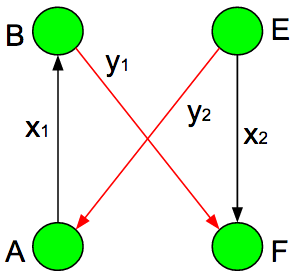
\includegraphics[height = 2.2cm, width = 2.5cm]{images/2opt.png}
\label{fig:2opt}
\caption{Illustration of Step 2(b) of 2-opt}
\end{figure}

Figure \ref{fig:2opt} is an example for $k$=2, where ($x_{1},y_{1}$) and ($x_{2},y_{2}$) are the pairs selected by Step 2(b). If $x_{1} + x_{2} > y_{1} + y_{2}$, then $x_{1}$ and $x_{2}$ will be exchanged with $y_{1}$ and $y_{2}$ at Step 3. \citep{LinKernighan73} perform several experiments and show that the value of $k$ has substantial influence on the performance of the algorithm and that the best choice for $k$ depends on the size of the TSP instance. Due to the importance of $k$, the algorithm is often referred to as \textit{k-opt}.

Additional refinements are added on top of the outlined steps of the algorithm. One of the refinements aims to minimise \textit{ checkout time}, which is the time spent between first encounter of an optimal tour $T$ and the second time the algorithm finds $T$ after exploring most options for tour improvement. The experiments have shown that this refinement is highly valuable, as on average 30 to 50 percent of computation time is spend on checkout time.

\subsection*{Empirical Analysis}
The algorithm was tested on 36 instances with up to 110 cities each\footnote{The upper bound on the city number is imposed due to computer storage limitations.}
 and it was let to run for time proportional to $\mathcal{O}(n^{2})$ iterations, where $n$ is the number of cities. \citet{LinKernighan73} observe that the frequency of finding an optimal tour is close to 1 for instances with up to 42 cities and for 100-city problems it drops to 0.2-0.3 on average\footnote{These numbers are derived only for the classical problems, where the optimal solution is known.}.

The algorithm was always able to find local optimum for all instances. This is a remarkable result. It shows that this algorithm is highly useful for cases when computation time is crucial and near-optimal solution is acceptable. 

The experiments show that as the allowed computation time is increased, the algorithm gives better solutions. This suggests that there is a trade off between running time and tour quality. 

The authors comment on the hardness of TSP instances involved in their experiment, a subject of research in later years for other NP-hard problems \citep{Cheeseman91, Ciaran16}. \citet{LinKernighan73} report that all problems are relatively easy, where random problems with distances not under the triangle are the hardest and the classical problems are the easiest.

Later work confirms the effectiveness of this algorithm for large TSPs \citep{Applegate03}. \citet{Applegate07} write that ``...at the heart of the most successful tour-finding approaches to date lies the simple and elegant algorithm of \citet{LinKernighan73}.''

\section{TSP and the Longest Path Problem}
\label{sec:tspandlpp}
A common way to solve a TSP instance $\pi$ is to reduce it to another problem $P$ for which there is a known efficient algorithm. Then, using the algorithm one solves $P$ and this gives the solution for $\pi$. This procedure is not equivalent to relaxation, since every solution to $P$ is a solution to $\pi$ and vice versa. This section is a review of a work by \citet{Hardgrave62} that makes a reduction from TSP to the Longest Path Problem (LPP). 

The Longest Path Problem (LPP) asks for finding a path between two specified vertices in a graph, such that the path has maximum length and does not contain any repeated vertices. LPP was not well researched at the time when \citet{Hardgrave62} was published and its NP-hadness was yet to be established \citep{thebible}. \citet{Hardgrave62} propose the following reduction from TSP to LPP with the hope that LPP ``... will prove to be easier ...'' than TSP.

A TSP instance can be represented as a directed labelled graph $G = (V,E, l)$, with a set of vertices $V=A$, a set of edges $E = \{(i,j) \,|\, i,j \in A \wedge i \neq j\}$ and a function $l$ that assigns a label on each edge, such that $\forall (i,j) \in E, \, l(i,j) = d_{i,j}$. A tour in TSP is then equivalent to a path in $G$ that visits each vertex once and returns to the starting city $v_{1}$. \citet{Hardgrave62} reduce TSP to LPP by showing that for every $G$ there exists a graph $L(G)$, such that a longest path in $L(G)$ corresponds to an optimal tour in $G$.

Graph $L(G)=(V^{\prime},E^{\prime},l^{\prime})$ has a set of vertices $V^{\prime}=V + a$, where  $a$ is an additional vertex, a set of edges $E^{\prime}$ that are the edges in $E$ except from the edges from any vertex to the start vertex, that is $(i,v_{1})$ plus edges $(i,v_{1})$ if and only if $(i,v_{1}) \in E$, and an edge labelling function $l^{\prime}$:

$l^{\prime}(i,j) = \begin{cases}
K - d_{i,j}, \quad \textrm{ if } j \neq v_{1} \\
K - d_{i,v_{1}}, \quad \textrm{ if } j = v_{1}, 
\end{cases}$

where $K$ is a constant that is strictly greater than the sum $S$ of the $n$ greatest distances $d_{i,j}$.

\begin{figure}
\centering
\begin{minipage}{.5\textwidth}
  \centering
  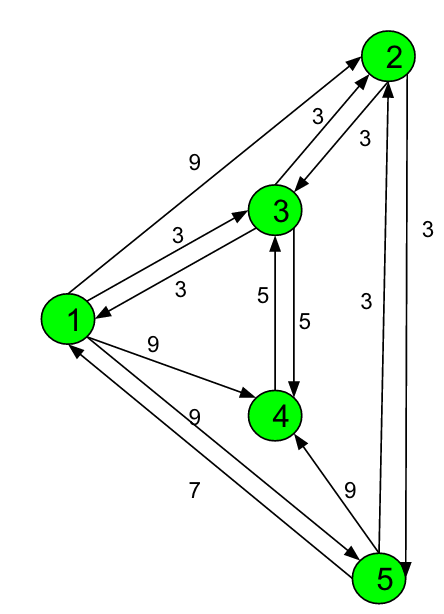
\includegraphics[width=4cm, height=5cm]{images/G.png}
\end{minipage}%
\begin{minipage}{.5\textwidth}
  \centering
  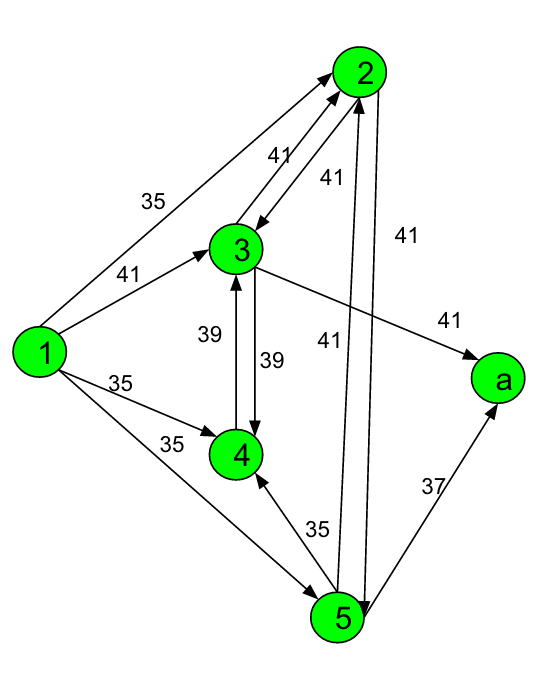
\includegraphics[width=4cm, height=5cm]{images/LG.png}
\end{minipage}
\label{fig:lgconstruction}
\caption{Construction of $L(G)$ from $G$, where $S=9+9+9+9+7=43$ and $K=44$}
\end{figure}

Figure \ref{fig:lgconstruction} is an example of $L(G)$, constructed from a particular graph $G$. An optimal tour in $G$ is $(1,4,3,2,5)$ and it is equivalent to the longest path in $L(G)$, which is $(1,4,3,2,5,a)$.

\citet{Hardgrave62} prove the correctness of the reduction and propose several procedures for solving LPP, which prove to be either not successful or inefficient. The proposed procedures are still useful for the research community as a guide of what ``not to do'' in order to solve LPP.

One of the ideas of \citet{Hardgrave62} is to find the longest spanning tree in $L(G)$ between $v_{1}$ and $a$, which is similar to the bounding procedure by \citet{HeldK71}, discussed earlier. \citet{Hardgrave62} are not clear about why this approach is unsuccessful. One of the suggested reasons is a failure to establish a method for choosing an initial spanning tree.

In summary, \citet{Hardgrave62} present an interesting idea of reducing an NP-hard problem to another NP-hard problem, with the hope that the latter problem will be easier to solve. They propose several procedures for solving LPP and give detailed explanation about why each of the procedures failed. \citet{Hardgrave62} do not provide a successful method for tackling TSP and LPP, but their work is a lesson about how certain procedures can lead to a dead-end.

\section{Conclusion}
The Travelling Salesman Problem (TSP) is a combinatorial optimisation problem that is applicable to multiple fields. This work introduced six influential approaches for solving TSP. Most of the methods implement similar ideas to the work of \citet{Dantzig54} \citep{Caseau97,HeldK71,Little63}. This shows that \citet{Dantzig54} is one of the fundamental works on TSP. This work showed that branch and bound algorithms are very effective techniques for solving TSP and demonstrated the flexibility of Constraint Programming for modelling optimisation problems.

This work reviewed a tour improvement algorithm for TSP by \citet{LinKernighan73}, which showed that it is often the case that an optimal or near-optimal solution is found relatively fast and most of the computation effort goes for proving that the solution is an optimum. This shows that tour-improvement techniques can significantly reduce the computation time and enable to solve substantially larger TSP instances, provided that a proof of their optimality is not required.

The reader should note that this work does not aim to present a review of the entire field of TSP. Due to the volume of existing work on TSP, that would prove impossible to do within a document of this size. The interested reader should refer to \citet{Applegate07,tspbible} for more detailed overview of TSP algorithms.

\newpage

% you should have a .bib file called mybibliographyfile.bib in the
% current directory for this to work
 \bibliographystyle{plainnat}
\bibliography{bibliography}

\end{document}
